\documentclass[11pt]{article}
\usepackage[margin=0.75in]{geometry}            % See geometry.pdf to learn the layout options. There are lots.
\geometry{letterpaper}                                  % ... or a4paper or a5paper or ...
%\geometry{landscape}                           % Activate for rotated page geometry
%\usepackage[parfill]{parskip}                  % Activate to begin paragraphs with an empty line rather than an indent
\usepackage{graphicx}                           % Use pdf, png, jpg, or eps§ with pdflatex; use eps in DVI mode
\usepackage{subcaption}
                                                                % TeX will automatically convert eps --> pdf in pdflatex
\usepackage{amssymb}
\usepackage{upquote}
\usepackage{multirow}
\usepackage{enumitem}
\usepackage{amsmath}
%-----------------------------------------------------------------------------
% Special-purpose color definitions (dark enough to print OK in black and white)
\usepackage{color}
% A few colors to replace the defaults for certain link types
\definecolor{orange}{cmyk}{0,0.4,0.8,0.2}
\definecolor{darkorange}{rgb}{.71,0.21,0.01}
\definecolor{darkgreen}{rgb}{.12,.54,.11}
%-----------------------------------------------------------------------------
% The hyperref package gives us a pdf with properly built
% internal navigation ('pdf bookmarks' for the table of contents,
% internal cross-reference links, web links for URLs, etc.)
\usepackage{hyperref}
\hypersetup{pdftex, % needed for pdflatex
  breaklinks=true, % so long urls are correctly broken across lines
  colorlinks=true,
  urlcolor=blue,
  linkcolor=darkorange,
  citecolor=darkgreen,
}


\title{Finance Project\\
  Stat 222, Spring 2016}

\author{
  Mingyung Kim, Weiyan Shi, Chih-Hui Wang
  \\
  \texttt{}
}

\begin{document}
\maketitle

\abstract{We model the spread crossing and mid-price movement of the Apple stock price using Support Vector Machine and Random Forest. Based on the predictions from both machine learning techniques, we design a trading strategy to gain profits in the stock market. Furthermore, because the interpretability of the machine learning method, we use the logistic regression to fit the data and try to figure out what features influence the stock price movement the most.}



\section{Introduction}
In this project, we explore the high-frequency trading activity in the stock market. The data is the limit order book of Apple on May 22nd, 2012. Our primary task is to predict and model the mid-price movement and spread crossing. Furthermore, we will use the model to develop the trading strategy and implement it using the real world data. We use Python to do the data preprocessing and modeling, especially scikit-learn \cite{scikit-learn}, and the ggplot2 package in R to do the visualization. The codes are all available in our Github repository \footnote{\url{https://github.com/jJasonWang/STAT_222_Finance}}.

In Section \ref{DataPreprocessing}, we explain how we extract the features from the limit order book and describe how we define the mid-price movement and spread crossing. For modeling, we mainly focus on Support Vector Machine (SVM) and Random Forest. In Section \ref{modelfitting}, we show the modeling procedures for both models. For Section \ref{modelassessment}, we present the evaluation of the model performance on the test set. One of the problems of machine learning algorithms is that they normally are hard to interpret, so we also fit the logistic model and try to explain some crucial features of the model which show in Section \ref{interpretation}. In Section \ref{strategy}, we implement our trading strategy based on the models and discuss the profit and potential drawback of the models. Finally, we will give an overall conclusion and discussion in Section \ref{conclusion}.



\section{Data Preprocessing} \label{DataPreprocessing}
\subsection{Feature Extraction}
We preprocess the given dataset into a data appropriate for our further modeling. We add features that can be useful for our prediction. We followed Kercheval and Zhang (2015) \cite{2015finance} and include the six feature vector sets as shown in Table \ref{tab:table1}. 

\begin{center}
  \captionof{table}{Feature Vector Sets} \label{tab:table1} 
  \begin{tabular}{|c | c |} 
    \hline
    Feature set & Description (\i=level index, n=10)\\
    \hline
    $v_{1}$=\{$P_{i}^{ask}$ , $V_{i}^{ask}$ , $P_{i}^{bid}$ , $V_{i}^{bid}$\} & price and volume (n levels)\\ 
    \hline
    $v_{2}$=\{(\ $P_{i}^{ask}$-$P_{i}^{bid}$ ) , (\ $P_{i}^{ask}$+$P_{i}^{bid}$ )/2\} & bid-ask spreads and mid-prices\\
    \hline
    $v_{3}$=\{(\ $P_{n}^{ask}$-$P_{1}^{ask}$ ) , (\ $P_{n}^{bid}$-$P_{1}^{bid}$ ) , $| P_{i+1}^{ask} - P_{i}^{ask} |$ , $| P_{i+1}^{bid} - P_{i}^{bid} |$\} & price differences \\
    \hline
    $v_{4}$=\{$\frac{1}{n}\ \sum_{i=1}^{n} P_{i}^{ask}$ , $\frac{1}{n}\ \sum_{i=1}^{n} P_{i}^{bid}$ , $\frac{1}{n}\ \sum_{i=1}^{n} V_{i}^{ask}$ , $\frac{1}{n}\ \sum_{i=1}^{n} V_{i}^{bid}$ \} & mean prices and volumes \\
    \hline
    $v_{5}$=\{$\sum_{i=1}^{n} (\ P_{i}^{ask}-P_{i}^{bid} )$ , $\sum_{i=1}^{n} (\ V_{i}^{ask}-V_{i}^{bid} )$\} & accumulated differences \\
    \hline
    $v_{6}$=\{$d P_{i}^{ask}$/$dt$ , $d P_{i}^{bid}$/$dt$ , $d V_{i}^{ask}$/$dt$ , $d V_{i}^{bid}$/$dt$\} & price and volume derivatives \\
    \hline
  \end{tabular}
\end{center}

Attributes in $v_{1}$ are prices and volumes up to n=10 levels at both ask and bid sides. They can be closely related to price movements. It is because investors make decisions based on prices and volumes and those decisions can affect price afterwards. Attributes in the $v_{2}$, $v_{3}$, $v_{4}$, $v_{5}$ are summary statistics (e.g. sum, mean, difference) of prices and be useful in predicting price movements. Of note is that the attributes except for those in $v_{6}$ are not dependent on time. We can consider the recent movements of prices and volumes by measuring the time-sensitive attributes in $v_{6}$. Those are average time derivatives of price and volume over the most recent one second. 



\subsection{Dependent Variables: Mid-price Movement and Spread Crossing}
Our first target is the mid-price movement. The mid-price of the stock is defined as the average of the best (highest) bid price and the best (lowest) ask price. At time $t$, we label the observation as up, stationary, or down if the mid-price at $t + \Delta t$ is bigger than, equal to, or smaller than the mid-price at $t$. We define time in terms of the number of time-stamped trade events. In the limit order book, each record represents one transaction. It may be the execution or cancellation of the market order. To balance the number of observation in each group, we choose $\Delta t$ equal to $10$ trading events, which, by using $\Delta t = 10$, the number of observations for up, stationary and down is around 1:1:1. 

Predicting spread crossing is our second goal. The spread crossing is up if the best bid price at $t + \Delta t$ is bigger than the best ask price at $t$. It is down if the best ask price at $t + \Delta t$ is larger than the best bid price at $t$. Otherwise, it is stationary. Same as the mid-price, we also define the time in term of the number of time-stamped trade events. When there is a movement for spreading crossing, it gives us the high chance to make a profit if predicted correctly in advance. For example, if we predict that the spread crossing is up at $t$, then we can buy the share at $t$ and sell them at $t + \Delta t$. The profit will be the difference between the best bid price at $t + \Delta t$ and the best ask price at $t$. Similarly, if the prediction at $t$ is down, we can short sell the share at $t$ and buy it back at $t + \Delta t$. To make the number of observations balanced across three categories, we set the $\Delta t$ as 1000.



\section{Model Fitting} \label{modelfitting}


For the model fitting, we split the dataset into two parts: 9:30 to 11:00 and 11:00 to 12:00. We use the first part of the dataset to train the model and assess the model performance. Then, we develop the trading strategy based on the model and implement on the second part of the dataset. The details of our trading strategy show in Section \ref{strategy}. There are 203,349 observations in the first part and 129,324 in the second part. 

We further split the first part of the dataset into three parts: training (50\%), validation (25\%) and testing sets (25\%). We use time order to separate the dataset. In other words, the first 50\% of the data will be in the train set, the next 25 \% of the data will be in the validation set, and the last 25\% of the data will be in the test set.  We use Figure \ref{fig:figure1} to summarize how we separate the data into different parts.

\begin{figure}
  \centering
    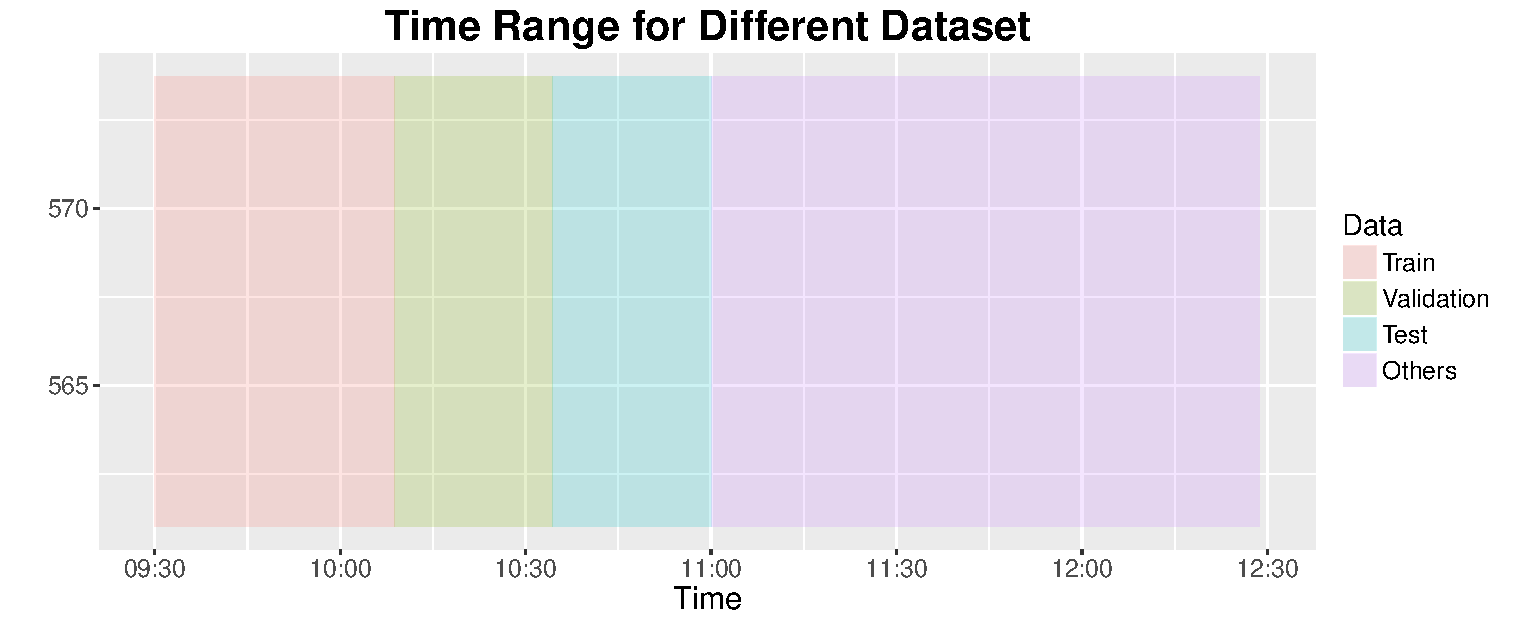
\includegraphics[width=0.8\textwidth]{Figures/TimeRange}
  \caption{Time Range for Different Dataset}
  \label{fig:figure1}
\end{figure}

We implement two machine learning techniques: Support Vector Machine (SVM) and Random Forest. To tune the parameters in each model, we fit the models with the different parameters for both machine learning methods on the training set and compare their performances on the validation set. Afterward, we can choose the optimal parameter based on the accuracy. Finally, we make the prediction on the testing set to present the model assessment.



\subsection{SVM}
For SVM, we use Gaussian kernel. The paper gives comprehensive explanations how SVM algorithm works, and we only focus on how we tune the parameters in this project. We have to tune two parameters $C$ and $\gamma$. The choice of the parameters shows the bias and variable trade-off for the model. If C is too large, the model will underfit the data which leads a wrong trading strategy. Similarly, if $\gamma$ is big, the decision boundary will be more smooth which indicates more bias and less variance.

We try $C=100, 1000, 10000$ and $\gamma=10^{-5}, 10^{-6}, 10^{-7}$ for both mid-price movement and spreading crossing. Since we have two parameters, we use the grid search to find the ideal pair of the parameters. In other words, we will fit a model for each pair of the parameter and compare their performances. However, due to the computational issue, we do not fit the model with the full training set. Instead, we use first 50,000 samples in the training set. We fit the model and tune the parameters for both mid-price movement and spread crossing. For the mid-price movement, it turns out that the optimal parameters are $C=100$ and $\gamma=10^{-6}$. Most of the accuracies are around 33\%. For the spread crossing, the optimal parameters are $C=1000$ and $\gamma=10^{-5}$. Most of the accuracies are around 35\%.



\subsection{Random Forest}
For the random forest, the parameters we need to select are the number of features in each split and number of trees. As the name suggest, the idea of random forest is to grow lots of trees. Each tree will make a prediction, and it will output the majority class as the predicted value. Also, to decorrelate the features, in each split of the tree, it only uses the subset of the features. Since we do not consider the full features set in each split, it makes the bias of the model increase. However, the number of trees will help us reduce the variance for the model. The effect of reducing variance will bring us some gains. Therefore, we need to choose an ideal pair of these two parameters.

For the number of features, we use two methods. The first one is $\log_2 m$ and the second is $\sqrt{m}$ where $m$ is the total number of features we have. On the other hand, for the number of trees, we try the numbers $50, 100, 200$. In general, the model performances remain the same after 200 trees, and the only cost for fitting many trees is computation. We do the grid search like SVM. Fitting the random forest seem to be not so time consuming as fitting SVM. We use the full training set for the random forest. For mid-price movement, the optimal number of features is $\sqrt{m}$ and the number of trees is $100$. It turns out that the optimal parameters for spreading crossing are the same as the one for mid-price movement.



\section{Model Assessment} \label{modelassessment}
To provide a complete picture of the models, we use precision, recall and F1-score to evaluate them. Table \ref{tab:cm} shows the confusion matrix and how to calculate those measures. The precision is the proportion of correct prediction when we predict positive, in our case: up, stationary or down. The recall is the correct prediction when the true label is positive. F1-score is an aggregate index combining measures. If all of them are close to 1, the model is great. Note that because our data have three classes: up, stationary, down, we transform the class into binary classes when we calculate the measures. That is, we will use the confusion matrix of up and not up when we calculate the precision for class up.

\begin{center}
\captionof{table}{Confusion Matrix for Binary Classification} \label{tab:cm}
\begin{tabular}{l|l|c|c|c}
\multicolumn{2}{c}{}&\multicolumn{2}{c}{True}&\\
\cline{3-4}
\multicolumn{2}{c|}{}&Positive&Negative\\
\cline{2-4}
\multirow{2}{*}{Predict}& Positive & True Positive & False Positive\\
\cline{2-4}
& Negative & False Negative & True Negative\\
\cline{2-4}
\end{tabular}
\end{center}

\newpage

\begin{itemize}
  \item $\mbox{Precision} = \frac{\mbox{True Positive}}{\mbox{True Positive + False Positive}}$
  \item $\mbox{Recall} = \frac{\mbox{True Positive}}{\mbox{True Positive + False Negative}}$
  \item $\mbox{F1-score} = \frac{\mbox{2 Precision}\times\mbox{Recall}}{\mbox{Precision + Recall}}$
\end{itemize}

\subsection{SVM}
For SVM, instead of refitting a model using all the train and validation data, we directly use the best model we found during the process of tuning parameters. That is, we only use 50,000 samples when we fit the model. We show the three measures of SVM model for mid-price movement in Table \ref{tab:svm1} and spread crossing in Table \ref{tab:svm2}. In fact, the model is not that much generalizable, and does not work well with the test data. We further check our confusion matrix and find out that for both cases, the SVM tends to make the prediction mainly on one class. That is why we observe the high recall in up class in each model.

\begin{center}
  \captionof{table}{Model Assessment for SVM: Mid-price Movement} \label{tab:svm1} 
  \begin{tabular}{|c | c | c | c|} 
    \hline
     & Precision & Recall & F1-score  \\
    \hline
    Up & 30.3\% & 33.8\% & 31.9\% \\ 
    \hline
    Stationary & 38.6\% & 0.164\% & 23.1\% \\
    \hline
    Down & 32.7\% & 51.3\% & 39.9\%  \\
    \hline
  \end{tabular}
\end{center}

\begin{center}
  \captionof{table}{Model Assessment for SVM: Spread Crossing} \label{tab:svm2} 
  \begin{tabular}{|c | c | c | c|} 
    \hline
    & Precision & Recall & F1-score \\
    \hline
    Up & 33.3\% & 20.2\%  & 25.2\% \\ 
    \hline
    Stationary & 38.7\% & 13.1\% & 19.6\% \\
    \hline
    Down & 34.9\% & 71.0\% & 46.8\%  \\
    \hline
  \end{tabular}
\end{center}

\subsection{Random Forest}
For the random forest, we refit the model on the train and validation data using the same parameters and make the prediction on the test data set. Table \ref{tab:rf1} shows the result for mid-price movement, and result for spread crossing is presented in Table \ref{tab:rf2}. It seems that the random forest can predict three classes but it does not predict very well with the new dataset.

\begin{center}
  \captionof{table}{Model Assessment for Random Forest: Mid-price Movement} \label{tab:rf1} 
  \begin{tabular}{|c | c | c | c|} 
    \hline
     & Precision & Recall & F1-score \\
    \hline
    Up & 40.7\%  & 46.5\% & 43.4\% \\ 
    \hline
    Stationary & 47.4\% & 15.8\% & 23.8\% \\
    \hline
    Down &  37.7\% & 62.2\%  & 46.9\%  \\
    \hline
  \end{tabular}
\end{center}

\begin{center}
  \captionof{table}{Model Assessment for Random Forest: Spread Crossing} \label{tab:rf2} 
  \begin{tabular}{|c | c | c | c|} 
    \hline
     & Precision & Recall & F1-score  \\
    \hline
    Up &  38.1\% & 28.5\% & 32.6\% \\ 
    \hline
    Stationary & 31.8\% & 22.2\% & 26.1\% \\
    \hline
    Down & 33.7\% & 52.1\% & 40.9\% \\
    \hline
  \end{tabular}
\end{center}

We try to figure out why our model perform so worse on the test dataset. As shown in the Figure \ref{figure3}. Actually, the movement for the data in the training set does not share the same trend as the data in the testing set. Besides, we do not include the time sensitive feature in our model. This is probably the reason why our model does not perform so well on the testing data.

\begin{figure}
  \centering
    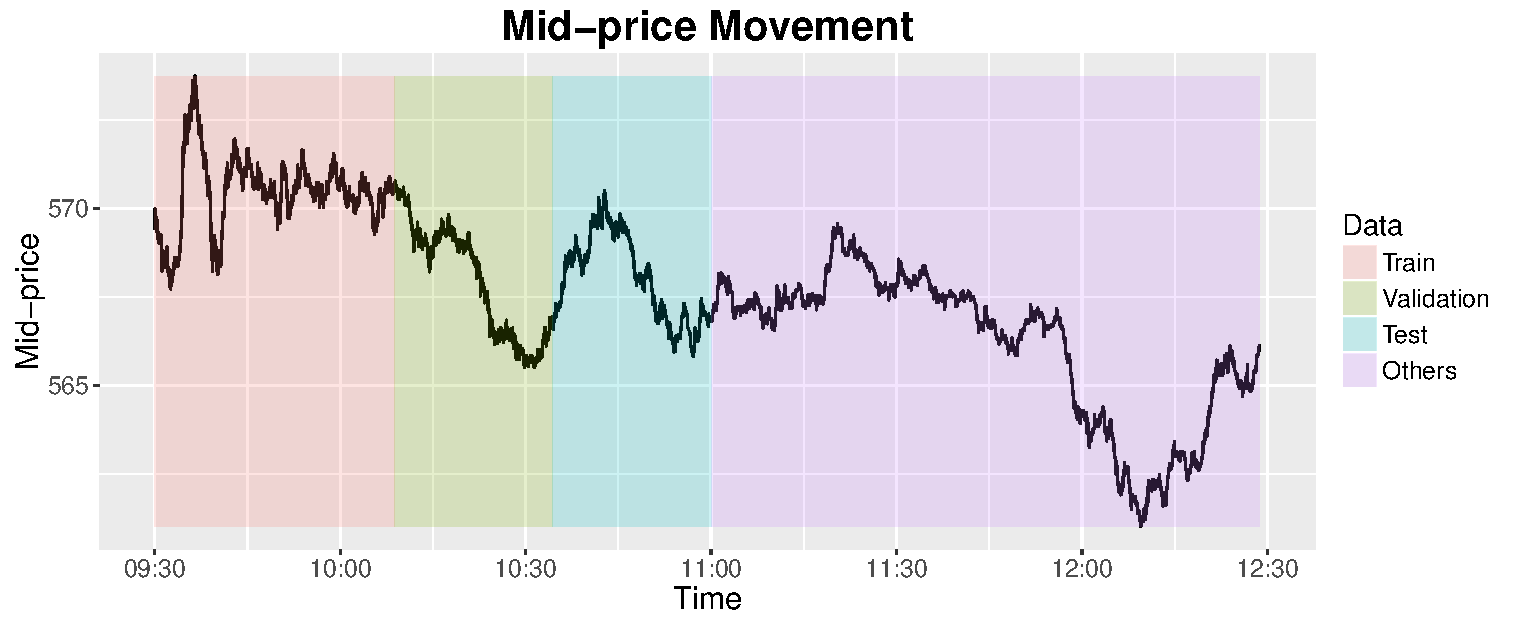
\includegraphics[width=0.8\textwidth]{Figures/Midprice}
  \caption{Mid-Price Movement}
  \label{figure2}
\end{figure}


\subsection{Feature Importances in Random Forest}
In this section, we show the feature importances in the random forest model for spread crossing. We can calculate the contribution of each feature based on the split made by that particular feature. In classification, we can use the reduced impurity as a measure to evaluate the importance or contribution of each feature. In regression, we can use the reduced variance to measure the feature importance. We show the features with top 10 high importances in Figure \ref{figure3}. In fact, most of the features contribute almost the same amount which means that they are equally important.

\begin{figure}
  \centering
    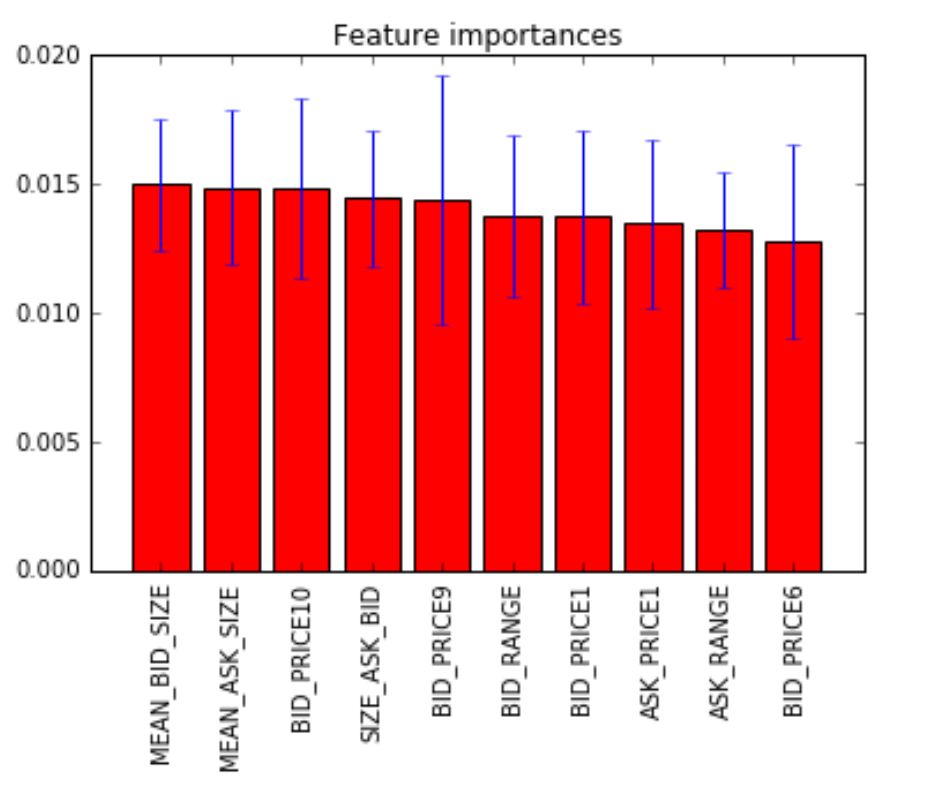
\includegraphics[width=0.6\textwidth]{Figures/importance}
  \caption{Feature Importances for Random Forest}
  \label{figure3}
\end{figure}


\section{Interpretation} \label{interpretation}
We come up with a new variable $v_{7}$  that can improve our prediction. The ratio of the total volume of top five ask-side orders and the total volume of top five bid-side orders can be an indication of the imbalance of supply and demand.

\begin{center}
  \captionof{table}{New Feature Set} \label{tab:tabv7} 
  \begin{tabular}{|c | c |} 
    \hline
    Feature set & Description (\i=level index, n=10)\\
    \hline
    $v_{7}$=\{$\sum_{i=1}^{5} V_{i}^{bid}$/$\sum_{i=1}^{5} V_{i}^{ask}$\} & volume ratio\\ 
    \hline
  \end{tabular}
\end{center}

We apply logistic regressions to predict the spread crossings. The equation is:

\begin{equation}
	\begin{split}
  y_{it} \sim Binary(p_{it}) \\
  logit(p_{it}) = \vec{\beta}^\top \vec{x_{it}} 
	\end{split}
\end{equation}

, where the dependent variables $y_{t}$ indicate dummy variables: (1) whether the spread crossing is up or not (i=1), (2) whether it is stationary or not (i=2), or (3) whether it is down or not (i=3) at time t. $x_{it}$ includes the six feature vectors in Table \ref{tab:table1} as well as the new feature in Table \ref{tab:tabv7}. 

We use the same model assessment measurements to compare with those obtained from the sophisticated model. By comparing Table \ref{tab:table1} with Tables \ref{tab:cm}-\ref{tab:rf2}, we find out that the prediction accuracy of the logistic regression model is not lower than that of the more sophisticated machine learning algorithms. The logistic model performs better than the other models in predicting the class "stationary" (Precision: 57.8\% for the logistic model, 38.6\% for SVM, 31.8\% for Random Forest).

\begin{center}
  \captionof{table}{Model Assessment for Logistic Model: Spread Crossing} \label{tab:table8} 
  \begin{tabular}{|c | c | c | c|} 
    \hline
     & Precision & Recall & F1-score  \\
    \hline
    Up &  8.7\% & 25.4\% & 12.9\% \\ 
    \hline
    Stationary & 57.8\% & 35.9\% &44.3\% \\
    \hline
    Down & 34.9\% & 32.8\% & 33.8\% \\
    \hline
  \end{tabular}
\end{center}

The logistic model also helps the interpretation of the results compared to the sophisticated machine learning algorithms with a strong black box flavor. Table 9 introduces the three variables that were estimated to have largest impacts on the spread crossings. The estimates of those variables were reported in parentheses. For example, the estimate of $d V_{1}^{ask}$/$dt$ is the largest with -0.0051 when we set dependent variable as a dummy variable whether the spread crossing is up or not. This result can be interpreted as: (1) $d V_{1}^{ask}$/$dt$ is the most important in predicting whether a spread crossing is up, (2) for a one-unit increase in $d V_{1}^{ask}$/$dt$, the expected change in log odds of having a up spread crossing is -0.0051. As we should interpret the coefficients using log odds, the interpretation may not be much intuitive compared to linear model. Still, the interpretation using the logistic model is much easier than that of the SVM and random forest.

One more interesting finding is that our new feature ($v_{7}$) works well in the logistic models for the stationary and down spread crossings. This feature is the second most important variable for those models. For example, the estimated $v_{7}$=$\sum_{i=1}^{5} V_{i}^{bid}$/$\sum_{i=1}^{5} V_{i}^{ask}$ is -0.0105 for the logistic regression model for up spread crossing. This means that the change in log odds of having downward spread crossing is expected to -0.0105, for a one-unit increase in $v_{7}$=$\sum_{i=1}^{5} V_{i}^{bid}$/$\sum_{i=1}^{5} V_{i}^{ask}$.  

\begin{center}
  \captionof{table}{Three Variables with the Largest Impacts on the Spread Crossing} \label{tab:title} 
  \begin{tabular}{|c | c | c | c|} 
    \hline
     & First & Second & Third  \\
    \hline
    Up & $d V_{1}^{ask}$/$dt$ (-0.0051) & $d V_{2}^{ask}$/$dt$ (-0.0046) & $d V_{5}^{ask}$/$dt$ (-0.0045)\\ 
    \hline
    Stationary & $\sum_{i=1}^{n} (\ P_{i}^{ask}-P_{i}^{bid} )$ (0.1871) & $\sum_{i=1}^{5} V_{i}^{bid}$/$\sum_{i=1}^{5} V_{i}^{ask}$ (0.0527) & $P_{10}^{ask}$-$P_{10}^{bid}$ (0.0231) \\
    \hline
    Down & $\sum_{i=1}^{n} (\ P_{i}^{ask}-P_{i}^{bid} )$ (-0.0741) & $\sum_{i=1}^{5} V_{i}^{bid}$/$\sum_{i=1}^{5} V_{i}^{ask}$ (-0.0105) & $P_{10}^{ask}$-$P_{10}^{bid}$ (-0.0099) \\
    \hline
  \end{tabular}
\end{center}

\section{Trading Strategy} \label{strategy}
To simplify the problem, we make the following assumptions:
\begin{enumerate}[label=(\alph*)]
\item There is no transaction cost.
\item We can place only market orders, and assume that they can be executed immediately at the best bid/ask.
\item The position can only be long/short at most one share.
\item We can only hold one share during the whole time period.
\end{enumerate}

We implement the same strategy for both SVM and random forest. And the strategy is:\\


\begin{center}
  \captionof{table}{Trading Strategy} \label{tab:title} 
  \begin{tabular}{|c | c | c | c|} 
    \hline
     & Meaning & Action & Profit \\
    \hline
    Up & ${P_{t+\Delta t}}^{bid} > {P_{t}}^{ask}$ & sell at $t+\Delta t$ & $Bid\_price1_{t+\Delta t} - Ask\_price1_t$ \\ 
    \hline
    Stationary &${P_{t+\Delta t}}^{bid} = {P_t}^{ask}$ &Do nothing & 0\\
    \hline
    Down &${P_{t}}^{bid} > {P_{t+\Delta t}}^{ask}$  & borrow a share at $t$, buy it back at $t+\Delta t$ & $Bid\_price1_{t} - Ask\_price1_{t+\Delta t}$ \\
    \hline
  \end{tabular}
\end{center}

Here is how we implement the strategy. We will start our transaction right at 11:00 am, and predict the label for the very first observation and then take some action according to the table above. Because we can only have one share at each timestamp, we have to sell/buy the share at $t+\Delta t$. From time t to time $t+\Delta t$, we could not take any action, so we have to jump to $t+\Delta t$ and predict the label for $t + \Delta t$. Then we move to $t+\Delta t$, so and so forth. In total, we would only have about 129 actions with 129,324 observations in total and $\Delta t$ to be 1000. For SVM, our profit is -\$20; for random forest, our profit is -\$24; for logistic regression, our profit is -\$12.

We have negative profit because the models didn't do well on the data after 11:00 am, we could see from the model assessment that all the classifiers are basically "guessing" the label. The logistic regression performs slightly better maybe because it performs better on predicting the "stationary" label with precision for class "stationary" being 57.8\%.

And one of the reasons why the models don't perform well on the data after 11:00am is because the pattern for the price after 11:00am is not similar at all to the data before 11:00am, we could see from Figure \ref{figure2} that after 11:00am, the price starts decreasing a lot. And because we didn't have many time-sensitive features in our dataset, we couldn't catch the downward trend. We could do some further improvements on that. In conclusion, using the data before 11:00am to build the model and predicting the labels after 11:00am is not a good idea.
 
\section{Conclusion} \label{conclusion}

In this project, we use the limit order book of Apple on May 22nd, 2012, and try to predict the mid-price movement and spread crossing. We choose the features that could help predict the two dependent variables. We first apply the sophisticated machine learning algorithms (e.g. SVM and Random Forest), evaluate model performances (e.g. precision, recall, F1-score), and measure the profits by implementing our strategies. We also fit the simple algorithm (e.g. logistic model) and compare the model performances as well as the profits with the sophisticated models. In fact, We can improve the interpretability without losing prediction accuracy or profits in a significant amount, by using a simple model.

Given the limitation of time and data, we do not improve the performance of the models much other than tuning the parameters. Moreover, because we do not have the sufficient knowledge about the data, the time-sensitive features are hard to implement. However, the time information of the stock is crucial for analysis. We can add more relevant features such as the lag of bid or ask price in the future to catch the time trend for the price movements, which may also be a potential way to improve our profit.

Besides, as said before, the data before 11:00 am is not a good indicator for the data after 11:00 am. One way to improve the profit is to combine different classifiers, make predictions and let them vote for the final predicted label. This method may increase our accuracy in the future and give us higher profit. Alternatively, we can use similar updating model strategy as did in Kercheval and Zhang (2015) \cite{2015finance} We keep update our model when we have a new observation. By doing so, we will capture the time trend of the data.

\newpage

\bibliography{Finance}{}
\bibliographystyle{unsrt}

\end{document}
